%  path0 <- "c:/data/NameRight/"; setwd(path <- paste0(path0, "program/"));  system("recycle c:/data/NameRight/program/cache/FirstYearDraft/"); library(knitr); knit("FirstYearDraft.rnw", "FirstYearDraft.tex"); system("platex FirstYearDraft"); system("pbibtex FirstYearDraft"); system("dvipdfmx FirstYearDraft")

\input{c:/migrate/R/knitrPreamble/knitr_preamble.rnw}
\makeatletter
\g@addto@macro{\UrlBreaks}{\UrlOrds}
\newcommand\gobblepars{%
    \@ifnextchar\par%
        {\expandafter\gobblepars\@gobble}%
        {}}
\makeatother
\def\pgfsysdriver{pgfsys-dvipdfm.def}
\usepackage{tikz}
\usetikzlibrary{calc, arrows, decorations, decorations.pathreplacing, backgrounds}
\usepackage{adjustbox}
\usepackage{longtable}
\usepackage[group-separator={,}, group-minimum-digits=4]{siunitx}
\renewcommand\Routcolor{\color{gray30}}
\renewcommand{\appendixname}{}

\tikzstyle{toprow} =
[
top color = gray!20, bottom color = gray!50, thick
]
\tikzstyle{maintable} =
[
top color = blue!1, bottom color = blue!20, draw = white
%top color = green!1, bottom color = green!20, draw = white
]
\tikzset{
%Define standard arrow tip
>=stealth',
%Define style for different line styles
help lines/.style={dashed, thick},
axis/.style={<->},
important line/.style={thick},
connection/.style={thick, dotted},
}


\begin{document}
\setlength{\baselineskip}{12pt}





\hfil Data and legal changes in women's name rights\\

\hfil\MonthDY\\
\hfil{\footnotesize\currenttime}\\
\renewcommand{\thefootnote}{*\arabic{footnote}}

\hfil Seiro Ito

\setcounter{tocdepth}{3}
\tableofcontents

\setlength{\parindent}{1em}
\vspace{2ex}


\section{Data}


















\subsection{Data source}

For the US, there are a few data sources on marriages and divorces. 
\begin{description}
\vspace{1.0ex}\setlength{\itemsep}{1.0ex}\setlength{\baselineskip}{12pt}
\item[NHGIS (IPUMS)]	Marriage related data sets. 
\item[NBER]	 A project that compiled marriage and divorce data between 1968-1988 {\footnotesize (\url{https://www.nber.org/research/data/marriage-and-divorce-data-1968-1995-0})}. Marriage data is individual couple entries of \num{12055875} cases. It is sample information and a sampling weight is attached to each entry.
\item[FRED]	FRED (data portal of St. Louis Fed) releases state level population estimates by year since 1900 {\footnotesize (\url{https://fred.stlouisfed.org/release/tables?rid=118&eid=259194&od=1960-01-01#} for 1960)}. The code is \texttt{SS}POP where \texttt{SS} is state FIPS code and can use API to download for all periods.
\item[SEER]	NIH-NCI (National Cancer Institutue) releases county level population (by age and sex) estimates between 1969-2020. {\footnotesize\url{https://seer.cancer.gov/popdata/download.html}}
\end{description}


\subsection{Plots}















\mpage{\textwidth}{
\hfil\textsc{Figure \refstepcounter{figure}\thefigure: Number of marriages by state (NBER)\label{NBER marriage}}\\
\hfil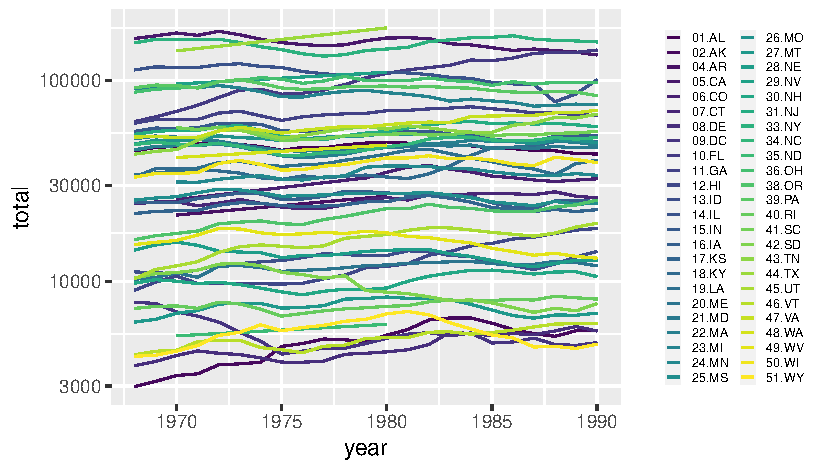
\includegraphics[width=.8\textwidth]{c:/data/NameRight/save/NumberOfMarriagesByState.pdf}\\
\hfil\begin{tabular}{>{\hfill\footnotesize }p{.1\textwidth}<{}>{\footnotesize }p{.8\textwidth}<{\hfill}}
Source: & NBER data.\\
Note: & \mpagethree{.8\textwidth}{\footnotesize Marriage information is partly sampled data. Sampling weights are used to obtain state level totals. }{t}
\end{tabular}
}

\vspace{4ex}
\mpage{\textwidth}{
\hfil\textsc{Figure \refstepcounter{figure}\thefigure: Number of divorces by state (NBER)\label{NBER divorce}}\\
\hfil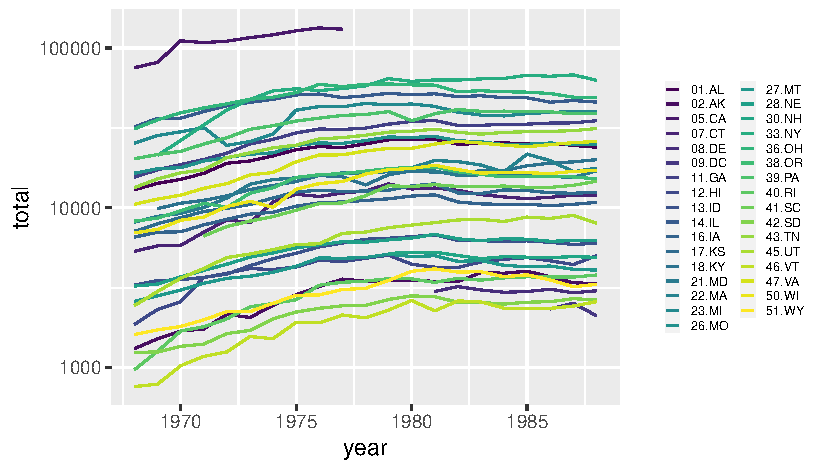
\includegraphics[width=.8\textwidth]{c:/data/NameRight/save/NumberOfDivorcesByState.pdf}\\
\hfil\begin{tabular}{>{\hfill\footnotesize }p{.1\textwidth}<{}>{\footnotesize }p{.8\textwidth}<{\hfill}}
Source: & NBER data.\\
Note: & \mpagethree{.8\textwidth}{\footnotesize Divorce information is partly sampled data. Sampling weights are used to obtain state level totals. }{t}
\end{tabular}
}

\vspace{2ex}
\mpage{.9\textwidth}{
\hfil\textsc{Figure \refstepcounter{figure}\thefigure: Marriage rate by state\label{marriage rate}}\\
\hfil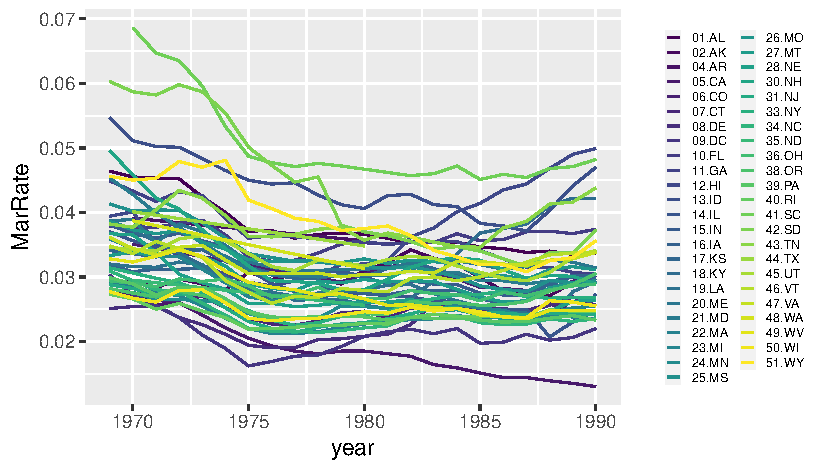
\includegraphics[width=.8\textwidth]{c:/data/NameRight/save/MarriageRateByState.pdf}\\
\hfil\begin{tabular}{>{\hfill\footnotesize }p{.1\textwidth}<{}>{\footnotesize }p{.8\textwidth}<{\hfill}}
Source: & NBER and SEER data.\\
Note: & \mpagethree{.8\textwidth}{\footnotesize Marriage rate is $\tfrac{\mbox{number of marriages}}{\mbox{youth population}}$. Youth population is sum of males and females of 15-40 years of age. Marriage information is partly sampled data. Sampling weights are used to obtain state level totals. Population data is based on Census Bureau data and adjustments are applied by NIH. }{t}
\end{tabular}
}

\vspace{4ex}
\mpage{.9\textwidth}{
\hfil\textsc{Figure \refstepcounter{figure}\thefigure: Divorce rate by state\label{divorce rate}}\\
\hfil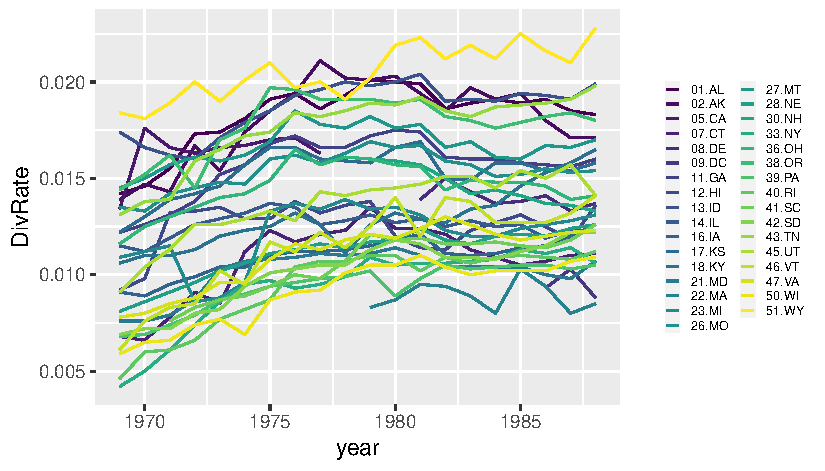
\includegraphics[width=.8\textwidth]{c:/data/NameRight/save/DivorceRateByState.pdf}\\
\hfil\begin{tabular}{>{\hfill\footnotesize }p{.1\textwidth}<{}>{\footnotesize }p{.8\textwidth}<{\hfill}}
Source: & NBER and SEER data.\\
Note: & \mpagethree{.8\textwidth}{\footnotesize Divorce rate is $\tfrac{\mbox{number of divorces}}{\mbox{youth population}}$. Youth population is sum of males and females of 15-40 years of age. Divorce information is partly sampled data. Sampling weights are used to obtain state level totals. Population data is based on Census Bureau data and adjustments are applied by NIH. }{t}
\end{tabular}
}

\vspace{2ex}
\mpage{.9\textwidth}{
\hfil\textsc{Figure \refstepcounter{figure}\thefigure: Marriage reporting by state\label{marriage reporting}}\\
\hfil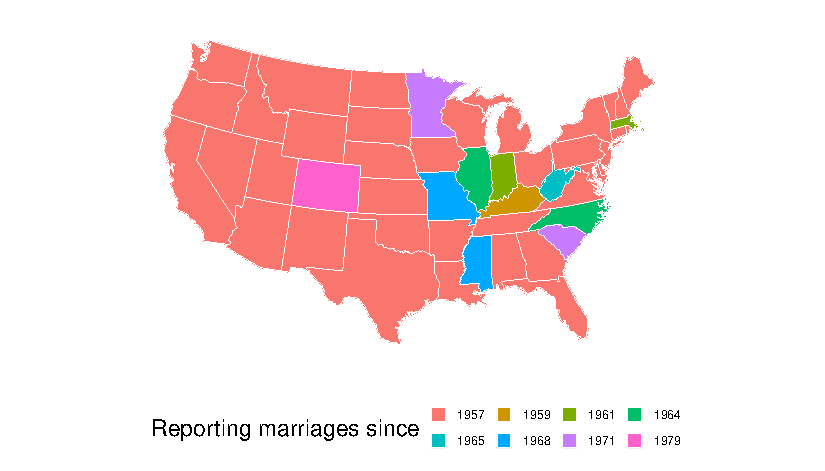
\includegraphics[width=.8\textwidth]{c:/data/NameRight/save/YearStartReportingMarriages.pdf}\\
\hfil\begin{tabular}{>{\hfill\footnotesize }p{.1\textwidth}<{}>{\footnotesize }p{.8\textwidth}<{\hfill}}
Source: & NBER data.\\
\end{tabular}
}

\vspace{4ex}
\mpage{.9\textwidth}{
\hfil\textsc{Figure \refstepcounter{figure}\thefigure: Divorce reporting by state\label{divorce reporting}}\\
\hfil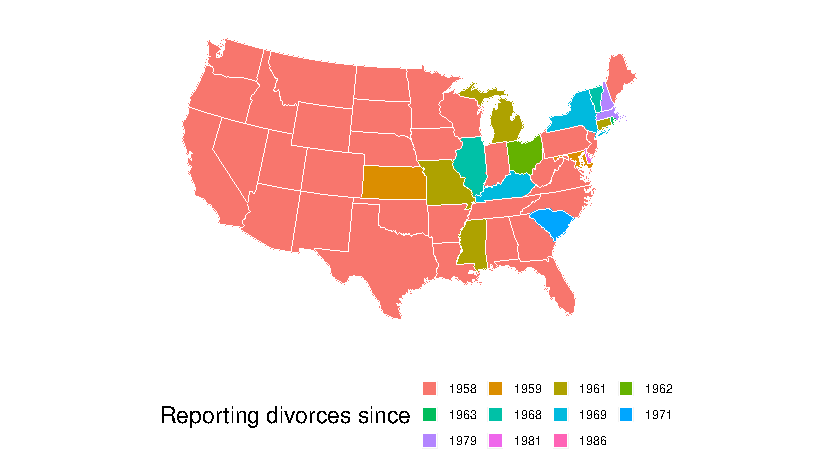
\includegraphics[width=.8\textwidth]{c:/data/NameRight/save/YearStartReportingDivorces.pdf}\\
\hfil\begin{tabular}{>{\hfill\footnotesize }p{.1\textwidth}<{}>{\footnotesize }p{.8\textwidth}<{\hfill}}
Source: & NBER data.\\
\end{tabular}
}

\vspace{4ex}
There are a few notable points we see in these figures:
\begin{itemize}
\vspace{1.0ex}\setlength{\itemsep}{1.0ex}\setlength{\baselineskip}{12pt}
\item	Irrespective of differences in sampling schemes (census vs. sample), the numbers broadly do not show jumps that may cause alerts. 
\item	Except for a few states, marriage and divorce reporting started well before the changes in women's name rights. Data coverage is long enough to pick up a change, or a lack thereof.
\item	Number of marriages (and divorces) are increasing due possibly to population growth.
\item	Economic downturns may cause marriages to decrease, as we see in 1975. Such a temporary decrease seems to be shared among all the states. 
\item	Economic downturns do not seem to decrease the number of divorces.
\item	When we look at ratios against youth population (defined as ages 15-40),  in the long run, marriage rates are decreasing while the divorce rates are increasing.
\end{itemize}




\section{Legal cases and political activities}

\subsection{Legal cases}



In the US before the 1960's, it was considered that women need to bear husbands' surnames. In \textit{Chapman v. Phoenix National Bank} of 1881\footnote{85 N.Y. 437, 449 (1881). The plaintiff purchased stock in the Phoenix National Bank before her marriage under her maiden name. When US Marshalls seized her asset, she sued on the ground that it held the assets under her maiden name, not her legal name, which is her husband's surname. NY Court of Appeals accepted the plaintiff's claim despite no reference to any law. }: 
\begin{quotation}
For several centuries, by the common law among all English speaking people, a woman, upon her marriage, takes her husband's surname. That becomes her legal name, and she ceases to be known by her maiden name. By that name she must sue and be sued, make and take grants and execute all legal documents. Her maiden surname is absolutely lost, and she ceases to be known thereby. 
\end{quotation}
The lack of legal foundation in this legal interpretation was explicitly noted in the 1960's as in State ex \textit{rel. Krupa v. Green}, 177 N.E. 2d 616, 619 (Ohio App. 8 Dist. 1961). In \textit{Forbush v. Wallace} of Alabama in 1971, the District Court for Middle District of Alabama's denied the woman's right to choose her maiden name upon obtaining driver's license, which was affirmed without a separate opinion by the Supreme Court in 1972. 

Possibly in tandem with this, in 1971, Department of State's position was negative on the right: ``[t]he legal name of a married woman is her husband's surname.'' In addition, to quote from \textit{Walker v. Jackson}, 391 F. Supp. 1395 (E.D. Ark. 1975), 
\begin{quotation}
[T]he Supreme Court of the United States has recognized that a State may constitutionally require a married woman to use her husband's surname as her own for certain purposes, as for example obtaining a driver's license, if the State has a sufficiently compelling interest in imposing the requirement. \textit{Forbush v. Wallace}, Governor, 405 U.S. 970, 92 S. Ct. 1197, 31 L. Ed. 2d 246 (1972), aff'g without opinion, \textit{Forbush v. Wallace}, Governor, 341 F. Supp. 217 (M.D.Ala.1971).
\end{quotation}


Such a position in public offices have slowly changed. According to \citet[][p.6]{Augustine1997}, legal challenges in the 1970's ``firmly establised that ... her name is unchanged by the fact that marriage had occurred.'' ``By the late 1970's and early 1980's many state legislatures codified a woman's right to name herself.'' 

\textsc{Table \ref{TabAFn18}} is tabulation of cases affirming women's name rights listed by \citet[][fn. 18]{Augustine1997}. The leading case was \textit{Dunn v. Palermo} in Tennessee (1975) that the State Supreme Court affirmed that women can register to vote under her maiden names. Additionally, in 1976, Florida District Court of Appeals noted that women are not compelled to change her name upon marriage (\textit{Marshall v. State}). Another leading case that recognizes the women's right to name is in Nebraska in 1978 (\textit{Simmons v. O'Brien}). In this case, the woman retained her former surnames during the marriage, then filed a divorce (marriage dissolution) to which the District Court denied the appeal because she did not file under husband's surname. The Trial Court reversed the District Court's decision and remanded with directions to accept the filing.

Other scholar notes that a decision in Alabama (\textit{Forbush v. Wallace}) of 1971 that denied the women's name right as a ``case inspired a great deal of subsequent litigation'' \citep[][299]{MacClintock2010}, a 1973 case in Maryland (\textit{Stuart v. Bd. of Supervisors of Elections for Howard County}) served as a guide, and a 1975 decision in Wisconsin (\textit{Kruzel v. Podell}) played a pivotal role across the US (\cite[][fn 4]{MacDougall1985}, \cite[][300]{MacClintock2010}). \textsc{Table \ref{TabMFn9}} lists all the formal cases and informal opinions by state judicial or state attorney generals affirming the right after 1972. In principle, one can date the year when the official common law practice shifted to affirm the right.\footnote{\href{https://law.justia.com/cases/federal/district-courts/FSupp/406/359/2143469/}{\textit{Allen v. Lovejoy}}, concluded in October 1975, however, notes that a woman who was suspended without pay due to noncompliance with Health Department's name change policy should not get compensation because she did not follow Department's advice to first change the name and appeal to the internal Merit System Council. Given the uncertainty of how MSC might have responded to plaintiff's appeal, the women's name right had not been fully protected until 1974 when the suspension was decided. } 

According to \citet[][p.8]{Augustine1997}, state legal codes have been ammended that a married woman has a right to retain her maiden name.\footnote{Louisiana is unique that it takes a civil law perspective that ``[m]arriage does not change the name of either spouse'' \citep[][p.8]{Augustine1997}. }





\begin{Schunk}
\begin{Soutput}

1931 1961 1972 1973 1974 1975 1976 1977 1978 1979 1980 1982 1983 1985 
   1    1    1    3   16   10    3    2    2    1    1    1    1    7 
\end{Soutput}
\end{Schunk}




\clearpage
\hfil\textsc{Table \refstepcounter{table}\thetable: References in \citet{Augustine1997}\label{TabAFn18}}\\
\setlength{\tabcolsep}{1pt}
\hfil\begin{longtable}{>{\hfill\footnotesize }p{3cm}<{}>{\hfill\footnotesize }p{3cm}<{}>{\hfil\footnotesize }p{2cm}<{}>{\footnotesize }p{0.75cm}<{}>{\footnotesize }p{5cm}<{}}
\rowcolor{lightblue}\makebox[3cm]{case} & \makebox[3cm]{ref} & \makebox[2cm]{state} & \makebox[0.75cm]{year} & \makebox[5cm]{remark}\\ \endfirsthead
\rowcolor{lightblue}\makebox[3cm]{case} & \makebox[3cm]{ref} & \makebox[2cm]{state} & \makebox[0.75cm]{year} & \makebox[5cm]{remark}\\ \endhead
Stuart v. Bd. of Supervisors of Elections for Howard County & 295 A.2d 223 & Maryland & 1972 & \mpage{5cm}{\footnotesize Holding that marriage did not, as a matter of law, change the wife's surname to that of the husband.\hfill\setlength{\baselineskip}{10pt}}\\\rowcolor{gray90}
Custer v. Bonadies & 318 A.2d 639 Conn. Super. Ct. & Connecticut & 1974 & \mpage{5cm}{\footnotesize Finding that neither common law nor statute compels a married woman to take her husband's surname, although it is the custom.\hfill\setlength{\baselineskip}{10pt}}\\
Marshall v. State & 301 So. 2d 477 Fla. Dist. Ct. App. & Florida & 1974 & \mpage{5cm}{\footnotesize Allowing a married woman to claim her nonmarital name as her legal name.\hfill\setlength{\baselineskip}{10pt}}\\\rowcolor{gray90}
In re Hauptly & 312 N.E.2d 857 & Indiana & 1974 & \mpage{5cm}{\footnotesize Holding that a married woman has the same right to change her name as anyone else.\hfill\setlength{\baselineskip}{10pt}}\\
MAss. Op. ATr'y GEN. & Number 5 at 48 & Massachusetts & 1974 & \mpage{5cm}{\footnotesize Finding that Massachusetts law does not compel a woman retaining her maiden name after marriage to assume her husband's surname for any purpose.\hfill\setlength{\baselineskip}{10pt}}\\\rowcolor{gray90}
In re Halligan & 361 N.Y.S.2d 458 App. Div. & New York & 1974 & \mpage{5cm}{\footnotesize Holding that the potential confusion which might arise when a woman bore a name different from her husband's was an insufficient reason to deny her application for judicial name change.\hfill\setlength{\baselineskip}{10pt}}\\
In re Natale & 527 S.W.2d 402, 404-05 Mo. Ct. App. & Montana & 1975 & \mpage{5cm}{\footnotesize Noting that restricting a woman's right to use the name of her choice is inconsistent with developments granting women equal legal rights.\hfill\setlength{\baselineskip}{10pt}}\\\rowcolor{gray90}
In re Lawrence & 337 A.2d 49, 51 N.J. Super. Ct. App. Div. & New Jersey & 1975 & \mpage{5cm}{\footnotesize Finding a "woman may retain her maiden name by antenuptial agreement or by holding herself out consistently by that name after marriage."\hfill\setlength{\baselineskip}{10pt}}\\
In re Mohlman & 216 S.E.2d 147 N.C. Ct. App. & North Carolina & 1975 & \mpage{5cm}{\footnotesize Stating that at marriage a woman does not give up her right to change her name as anyone else might change his or hers.\hfill\setlength{\baselineskip}{10pt}}\\\rowcolor{gray90}
In re Strikwerda & 220 S.E.2d 245 & Verginia & 1975 & \mpage{5cm}{\footnotesize Finding that nothing in the wording of statute purports to exclude a married woman from petitioning the court to change her name from her married name to her maiden name.\hfill\setlength{\baselineskip}{10pt}}\\
Kruzel v. Podell & 226 N.W.2d 458,459 & Wisconsin & 1975 & \mpage{5cm}{\footnotesize Finding error in an election board's purging of voter registration where a woman did not take her husband's surname at marriage.\hfill\setlength{\baselineskip}{10pt}}\\\rowcolor{gray90}
Weathers v. Superior Court of Los Angeles & 126 Cal. Rptr. 547 Ct. App. & California & 1976 & \mpage{5cm}{\footnotesize Allowing a married woman to sue for divorce in her own name.\hfill\setlength{\baselineskip}{10pt}}\\
FLA. ATr'y GEN. ANN. REP. & \textsection 076-66  at 120 & Florida & 1976 & \mpage{5cm}{\footnotesize Advising that for purposes of voter registration, the "true" name of a married woman who chooses to retain her birth surname is her given name and her birth surname, not her given name and her husband's surname.\hfill\setlength{\baselineskip}{10pt}}\\\rowcolor{gray90}
Brown v. Brown & 384 A.2d 632, 632 & District of Columbia & 1977 & \mpage{5cm}{\footnotesize Finding no limitation in the common law for "any adult or emancipated person" to change his or her name at will.\hfill\setlength{\baselineskip}{10pt}}\\
Secretary of the Commonwealth v. City Clerk of Lowell & 366 N.E.2d 717 & Massachusetts & 1977 & \mpage{5cm}{\footnotesize Recognizing that a woman may change her name at will, without resort to legal proceedings.\hfill\setlength{\baselineskip}{10pt}}\\\rowcolor{gray90}
Ball v. Brown & 450 F. Supp. 4 N.D. & Ohio & 1977 & \mpage{5cm}{\footnotesize Finding error in an election board's purging of voter registration where a woman did not take her husband's surname at marriage.\hfill\setlength{\baselineskip}{10pt}}\\
ME. Op. ATr'Y GEN. & WL 33940 Me.A.G. & Maine & 1978 & \mpage{5cm}{\footnotesize Ruling that both women and men have option of retaining their surnames after marriage.\hfill\setlength{\baselineskip}{10pt}}\\\rowcolor{gray90}
Simmons v. O'Brien & 272 N.W.2d 273 & Nebraska & 1978 & \mpage{5cm}{\footnotesize Finding error in lower court's refusal to grant a divorce in wife's separate surname because common law did not compel married woman to bear the same surname as her husband.\hfill\setlength{\baselineskip}{10pt}}\\
In re Miller & 243 S.E.2d 464 & Verginia & 1978 & \mpage{5cm}{\footnotesize Noting that no statute in Virginia requires a married woman to assume her husband's surname, despite custom.\hfill\setlength{\baselineskip}{10pt}}\\\rowcolor{gray90}
Traugott v. Petit & 404 A.2d 77 & Rhode Island & 1979 & \mpage{5cm}{\footnotesize Upholding the common law right of a divorced woman to use the name of her choice.\hfill\setlength{\baselineskip}{10pt}}\\
Malone v. Sullivan & 605 P.2d 447 & Arizona & 1980 & \mpage{5cm}{\footnotesize Finding error in a trial court's refusal to entertain a woman's divorce petition unless she amended her pleading to reflect her surname as her husband's.\hfill\setlength{\baselineskip}{10pt}}\\\rowcolor{gray90}
State v. Taylor & 415 So. 2d 1043, 1047 & Alabama & 1982 & \mpage{5cm}{\footnotesize Finding that "in view of the fact that the common law regarding 'names' has not been altered by the legislature." Alabama adopts the common law of England that a woman's change of name upon marriage is in fact rather than in law.\hfill\setlength{\baselineskip}{10pt}}\\
\end{longtable}


\hfil\begin{tabular}{>{\hfill\footnotesize }p{.1\textwidth}<{}>{\footnotesize }p{.8\textwidth}<{\hfill}}
Source: & \citet{Augustine1997}\\
Note: & Legal cases and opinions endorsing the women's name rights are listed. 
\end{tabular}
\vspace{4ex}

\clearpage
\setcounter{table}{1}
\hfil\textsc{Table \refstepcounter{table}\thetable: References in \citet{MacDougall1985}\label{TabMFn9}}\\
\setlength{\tabcolsep}{1pt}
\hfil\begin{longtable}{>{\hfill\footnotesize }p{2.5cm}<{}>{\footnotesize }p{0.75cm}<{}>{\footnotesize }p{4cm}<{}>{\footnotesize }p{6cm}<{}}
\rowcolor{lightblue}\makebox[2.5cm]{state} & \makebox[0.75cm]{year} & \makebox[4cm]{case} & \makebox[6cm]{reference}\\ \endfirsthead
\rowcolor{lightblue}\makebox[2.5cm]{state} & \makebox[0.75cm]{year} & \makebox[4cm]{case} & \makebox[6cm]{reference}\\ \endhead
Alabama & 1982 & State v. Taylor & 415 So. 2d 1043 (Ala. 1982)\\\rowcolor{gray90}
Alaska & 1976 & Op. Att'y. Gen. & Alaska (May 5, 1976)\\
Arizona & 1975 & Laks v. Laks & 25 Ariz. App. 58, 540 P.2d 1277 (1975) [Seiro added: Divorced mother's right to rename children as MotherMaidenName-FatherSurName was rejected by the court.]\\\rowcolor{gray90}
Arizona & 1980 & Malone v. Sullivan & 124 Ariz. 469, 605 P.2d 447 (1980)\\
Arkansas & 1974 & Op. Att'y Gen. & Ark. No. 74-123 (Oct. 8, 1974) [Seiro added: Under Arkansas law a married woman may retain her maiden name, and if Pamela Walker did not change her name when she married she was entitled to be registered under her maiden name. \url{https://law.justia.com/cases/federal/district-courts/FSupp/391/1395/1494569/}]\\\rowcolor{gray90}
Arkansas & 1974 & Op. Att'y Gen. & Ark. No. 74-75 (April 19, 1974)\\
Arkansas & 1975 & Walker v. Jackson & 391 F. Supp. 1395 (E.D. Ark. 1975)\\\rowcolor{gray90}
California & 1974 & Op. Atty Gen. & Cal. (March 12, 1974)\\
California & 1976 & Weathers v. Superior Court & 54 Cal. App. 3d 286, 126 Cal. Rptr. 547 (1976)\\\rowcolor{gray90}
Connecticut & 1974 & Custer v. Bonadies & 30 Conn. Supp. 385, 318 A.2d 639 (Super. Ct. 1974)\\
Connecticut & 1975 & Op. Att'y Gen. & Conn. (Jan. 23, 1975)\\\rowcolor{gray90}
Delaware & 1974 & Op. Att'y Gen. & Del. (Aug. 7, 1974)\\
District of Columbia & 1975 & Op. Corp. Counsel D.C. & (1975)\\\rowcolor{gray90}
District of Columbia & 1978 & Brown v. Brown & 382 A.2d 1038 (D.C. 1978), vacating 384 A.2d 632 (D.C. 1977)\\
Florida & 1974 & Marshall v. State & 301 So. 2d 477 (Fla. Dist. Ct. App. 1974)\\\rowcolor{gray90}
Florida & 1976 & Davis v. Roos & 326 So. 2d 226 (Fla. Dist. Ct. App. 1976)\\
Florida & 1976 & 1976 Op. Att'y Gen. & Fla. 076-66 (March 24, 1976)\\\rowcolor{gray90}
Florida & 1983 & In re Hooper & 436 So. 2d 401 (Fla. Dist. Ct. App. 1983)\\
Florida & 1984 & Pilch v. Pilch & 447 So. 2d 989 (Fla. Dist. Ct. App. 1984)\\\rowcolor{gray90}
Georgia & 1975 & Op. Att'y Gen. & Ga. No. 75-49 (June 3, 1975)\\
Georgia & 1985 & Ga. Code Ann. & \textsection 19-3-33.1 (Supp. 1985)\\\rowcolor{gray90}
Hawaii & 1976 & Hawaii Rev. Stat. & \textsection 574-1 (1976)\\
Hawaii & 1979 & Jech v. Burch & 466 F. Supp. 714 (D. Hawaii 1979)\\\rowcolor{gray90}
Illinois & 1974 & Op. Att'y Gen. & Ill. No. S-711 (Feb. 25, 1974)\\
Illinois & 1974 & Op. Att'y Gen. & Ill. S-695 (Feb. 13, 1974), both opinions indicating that Illinois does not follow Rago v. Lipsky, 327 Ill. App. 63, 63 N.E.2d 642 (1945) (country's sole case holding that a married woman takes her husband's surname as her "legal" name at common law)\\\rowcolor{gray90}
Indiana & 1974 & In re Hauptly & 262 Ind. 150, 312 N.E.2d 857 (1974)\\
Iowa & 1980 & Op. Att'y Gen. & Iowa (March 25, 1980)\\\rowcolor{gray90}
Iowa & 1981 & Iowa Code Ann. & \textsection 595.5 (West 1981)\\
Kansas & 1973 & Op. Att'y Gen. & Kan. No. 73-47 (Feb. 1, 1973) following Gallop v. Shanahan No. 120, 456 (Dist. Ct. Shawnee County, Nov. 2, 1972), noted in Note, Constitutional Law-Equal Protection and Right of Suffrage Prohibits State From Cancelling Voter Registration of Newly Married Woman-Women Upon Marriage Do Not Necessarily Abandon Maiden Name, 21 U. Kan. L. Rev. 588 (1972-73)\\\rowcolor{gray90}
Kentucky & 1974 & Op. Att'y Gen. & Ky. No. 74-902 (Dec. 26, 1974)\\
Kentucky & 1974 & Op. Att'y Gen. & Ky. No. 74-349 (May 14, 1974)\\\rowcolor{gray90}
Kentucky & 1977 & Op. Att'y Gen. & Ky. No. 77-334 (May 23, 1977)\\
Kentucky & 1977 & Op. Att'y Gen. & Ky. No. 77-239 (April 13, 1977)\\\rowcolor{gray90}
Kentucky & 1981 & Memorandum Ky. Dept. Transportation & (Oct. 30, 1981) (Kentucky Department of Transportation relinquishes position that a married woman must obtain driver's license in her husband's surname unless she has a court-ordered name "change")\\
Louisiana & 1931 & Succession of Kneipp & 172 La. 411, 134 So. 376 (1931)\\\rowcolor{gray90}
Louisiana & 1975 & Boothe v. Papale & No. 74-939 (E.D. La. Feb. 12, 1975) (Order granting plaintiffs Motion for Summary Judgment) [Seiro added: Affirms that, in Lousiana, it is customary for women to use the maiden name after marriage. \citep[][fn 54]{Gorence1976}]\\
Louisiana & 1977 & Pugh v. Theall & 342 So. 2d 274 (La. Ct. App. 1977), cert. denied 344 So. 2d 1055 (La. 1977) [Seiro added: Affirms that, in Lousiana, it is customary for women to use the maiden name after marriage. \url{https://www.casemine.com/judgement/us/591494baadd7b049345c1e1e}]\\\rowcolor{gray90}
Louisiana & 1984 & La. Rev. Stat. Ann. & \textsection 40:34.A.(1)(a)(iii) (West 1984) (statute relating to naming children at birth)\\
Maine & 1974 & Op. Atty. Gen. & Me. (April 12, 1974)\\\rowcolor{gray90}
Maine & 1975 & In re Reben & 342 A.2d 688 (Me. 1975)\\
Maine & 1978 & Op. Att'y Gen. & Me. (April 4, 1978)\\\rowcolor{gray90}
Maryland & 1972 & Stuart v. Board of Supervisors & 266 Md. 440, 295 A.2d 223 (1972), noted in The Right of a Married Woman To Use Her Birth-Given Surname For Voter Registration, 32 Md. L. Rev. 409 (1973)\\
Maryland & 1972 & Op. Att'y Gen. & Md. (Nov. 30, 1972)\\\rowcolor{gray90}
Maryland & 1974 & Op. Att'y Gen. & Md. (May 7, 1974)\\
Maryland & 1974 & Op. Atty. Gen. & Md.(March 30, 1974)\\\rowcolor{gray90}
Maryland & 1977 & Klein v. Klein & 36 Md. App. 177, 373 A.2d 86 (Ct. Spec. App. 1977)\\
Maryland & 1981 & Goldin v. Goldin & 48 Md. App. 154, 426 A.2d 410 (Ct. Spec. App. 1981)\\\rowcolor{gray90}
Maryland & 1983 & Op. Att'y Gen. & Md. (Jan. 20, 1983)\\
Massachusetts & 1977 & Secretary of the Commonwealth v. City Clerk of Lowell & 373 Mass. 178, 366 N.E.2d 717 (1977)\\\rowcolor{gray90}
Massachusetts & 1983 & Mass. Ann. & Laws ch. 46 \textsection 1D (Law. Co-op. Supp. 1983)\\
Michigan & 1974 & Op. Att'y Gen. & Mich. No. 4834 (Oct. 2, 1974)\\\rowcolor{gray90}
Michigan & 1976 & Piotrowski v. Piotrowski & 71 Mich. App. 213, 247 N.W.2d 354 (1976)\\
Michigan & 1980 & Wood v. Detroit Edison & 409 Mich. 279, 294 N.W.2d 571 (1980)\\\rowcolor{gray90}
Michigan & 1980 & Mich. Comp. Laws Ann. & \textsection 333.2824(1) (West 1980) (statute relating to naming children at birth)\\
Michigan & 1983 & Jones v. Sanilac County Road Comm'n & 128 Mich. App. 569, 342 N.W.2d 532 (1983)\\\rowcolor{gray90}
Minnesota & 1985 & Minn. Stat. Ann. & \textsection 517.08 (West Supp. 1985)\\
Missouri & 1975 & In re Natale & 527 S.W.2d 402 (Mo. Ct. App. 1975)\\\rowcolor{gray90}
Missouri & 1983 & Johnson v. Pacific Intermountain Expr. Co. & 662 S.W.2d 237 (Mo. 1983), cert denied 104 S. Ct. 2349 (1984)\\
Missouri & 1984 & Miller v. Miller & 670 S.W.2d 591 (Mo. Ct. App. 1984)\\\rowcolor{gray90}
Montana & 1974 & Op. Att'y Gen. & Mon. (May 1, 1974)\\
Nebraska & 1978 & Simmons v. O'Brien & 201 Neb. 778, 272 N.W.2d 273 (1978)\\\rowcolor{gray90}
Nebraska & 1984 & Neb. Rev. Stat. & \textsection 71-640.01 (1984) (statute relating to naming children at birth)\\
New Hampshire & 1978 & Moskowitz v. Moskowitz & 118 N.H. 199, 385 A.2d 120 (1978)\\\rowcolor{gray90}
New Hampshire & 1983 & N.H. Rev. Stat. Ann. & \textsection 126.6-a (1983) (statute relating to naming children at birth)\\
New Jersey & 1975 & In re Lawrence & 133 N.J. Super. 408, 337 A.2d 49 (1975)\\\rowcolor{gray90}
New Jersey & 1975 & Op. Att'y Gen. & N.J. No. 20-1975 (Aug. 26, 1975)\\
New York & 1974 & In re Halligan & 46 A.D.2d 170, 361 N.Y.S.2d 458 (App. Div. 1974)\\\rowcolor{gray90}
New York & 1985 & N.Y. Dom. Rel. Law & \textsection\textsection 14-a(1), 15(1), 240-a (McKinney Supp. 1985)\\
New York & 1985 & N.Y. Civ. Rights Law & \textsection\textsection 64, 65 (McKinney Supp. 1985)\\\rowcolor{gray90}
North Carolina & 1975 & In re Mohlman & 26 N.C. App. 220, 216 S.E.2d 147 (1975)\\
North Carolina & 1981 & O'Brien v. Tilson & 523 F. Supp. 494 (E.D.N.C. 1981)\\\rowcolor{gray90}
North Carolina & 1983 & N.C. Gen. & Stat. \textsection 130-A-101(c) (Supp. 1983) (statute relating to naming children at birth)\\
North Dakota & 1974 & Op. Att'y Gen. & N.D. (March 20, 1974)\\\rowcolor{gray90}
Ohio & 1961 & Krupa v. Green & 144 Ohio App. 497, 177 N.E.2d 616 (1961)\\
Ohio & 1977 & Ball v. Brown & 450 F. Supp. 4 (N.D. Ohio 1977)\\\rowcolor{gray90}
Oklahoma & 1975 & Op. Att'y Gen. & Okla. (Nov. 14, 1975)\\
Oklahoma & 1978 & Sneed v. Sneed & 585 P.2d 1363 (Okla. 1978)\\\rowcolor{gray90}
Oregon & 1983 & Ore. Rev. Stat. & \textsection 106.220 (1983)\\
Pennsylvania & 1973 & Op. Att'y Gen. & Pa. No. 72 (Oct. 25, 1973)\\\rowcolor{gray90}
Pennsylvania & 1973 & Op. Att'y Gen. & Pa. No. 62 (Aug. 20, 1973)\\
Pennsylvania & 1974 & Op. Att'y Gen. & Pa. No. 8 (Jan. 31, 1974)\\\rowcolor{gray90}
Rhode Island & 1979 & Traugott v. Petit & 122 R.I. 60, 404 A.2d 77 (1979)\\
South Carolina & 1974 & Op. Att'y Gen. & S.C. (Dec. 12, 1974)\\\rowcolor{gray90}
South Carolina & 1975 & Op. Atty. Gen. & S.C. (June 6, 1975)\\
South Dakota & 1977 & Op. Att'y Gen. & S.D. No. 77-31 (April 15, 1977) (interpreting Ogle v. Circuit Court 89 S.D. 18, 227 N.W.2d 621 (1975))\\\rowcolor{gray90}
Tennessee & 1975 & Dunn v. Palermo & 522 S.W.2d 679 (Tenn. 1975)\\
Tennessee & 1983 & Tenn. Code Ann. & \textsection 68-3-305 (1983) (statute relating to naming children at birth)\\\rowcolor{gray90}
Texas & 1897 & Rice v. State & 37 Tex. Crim. 36, 38 S.W. 801 (1897)\\
Texas & 1974 & Op. Att'y Gen. & Tex. No. H-432 (Oct. 25, 1974)\\\rowcolor{gray90}
Texas & 1980 & Op. Att'y Gen. & Tex. No. MW-225 (Aug. 21, 1980) (says that a married woman may vote under a hyphenated last name, of her "maiden name" and her husband's name)\\
Vermont & 1974 & Op. Att'y Gen. & Vt. No. 179 (Feb. 4, 1974)\\\rowcolor{gray90}
Virginia & 1973 & Op. Att'y Gen. & Va. (June 6, 1973) (re voting)\\
Virginia & 1975 & In re Strikwerda & 216 Va. 470, 220 S.E.2d 245 (1975)\\\rowcolor{gray90}
Virginia & 1978 & In re Miller & 218 Va. 939, 243 S.E.2d 464 (1978)\\
Washington & 1927 & Op. Att'y Gen. & Wash. 507 (1927-28) (right of married woman to use husband's name even though she is not living with him)\\\rowcolor{gray90}
Washington & 1976 & Doe v. Dunning & 87 Wash. 2d 50, 549 P.2d 1 (1976)\\
West Virginia & 1975 & Op. Att'y Gen. & W. Va. (April 30, 1975)\\\rowcolor{gray90}
Wisconsin & 1975 & Kruzel v. Podell & 67 Wis. 2d 138, 226 N.W.2d 458 (1975)\\
Wisconsin & 1977 & Op. Att'y Gen. & Wis. No. 7-77 (Jan. 31, 1977)\\\rowcolor{gray90}
Wisconsin & 1982 & Op. Att'y Gen. & Wis. (Sept. 21, 1982)\\
\end{longtable}


\hfil\begin{tabular}{>{\hfill\footnotesize }p{.1\textwidth}<{}>{\footnotesize }p{.8\textwidth}<{\hfill}}
Source: & \citet{MacDougall1985}.\\
Note: & Legal cases and opinions endorsing the women's name rights are listed. Some negative cases are also listed for earlier dates. The six states not listed, Colorado, Idaho, Nevada, New Mexico, Utah, and Wyoming, all recognize the right but have not circulated the opinions by 1985. State level recognition of women's name right led to a federal level concensus in 1982 that women should not be denied to open financial accounts under her birth-given surname as an interpretation of Equal Opportunity Credit Act [\href{https://www.ecfr.gov/current/title-12/chapter-II/subchapter-A/part-202/section-202.7#p-202.7(b)}{12 C.F.R. \textsection 202.7 (b) Designation of names}].
\end{tabular}

\mpage{.9\textwidth}{
\hfil\textsc{Figure \refstepcounter{figure}\thefigure: First legal decision/opinion affirming the right by state\label{first legal}}\\
\hfil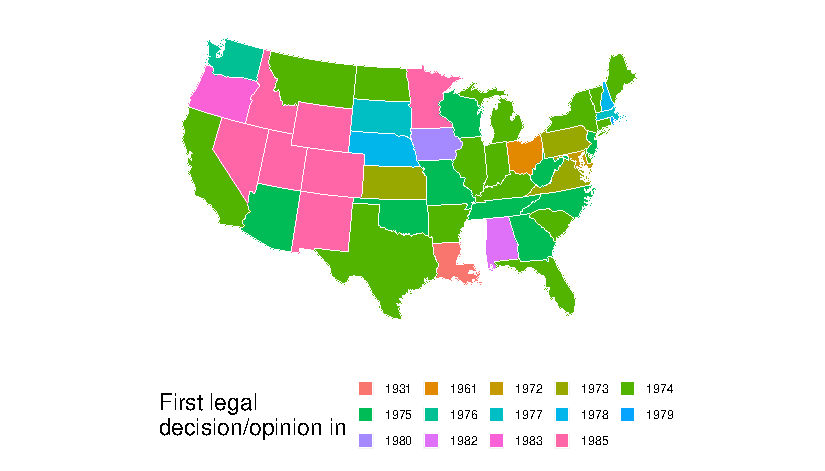
\includegraphics[width=.8\textwidth]{c:/data/NameRight/save/YearOfFirstLegalOpinionDecision.pdf}\\
\hfil\begin{tabular}{>{\hfill\footnotesize }p{.1\textwidth}<{}>{\footnotesize }p{.8\textwidth}<{\hfill}}
Source: & Author's compilation based on \citet[][fn 9]{MacDougall1985}.\\
Note: & The six states, Colorado, Idaho, Nevada, New Mexico, Utah, and Wyoming, are displayed as 1985 for expositional convenience. They all recognize the right but have not circulated the opinions by 1985. Mississippi is not listed in \citet[][fn 9]{MacDougall1985} and is left as blank.
\end{tabular}
}

\vspace{4ex}
\textsc{Figure \ref{first legal}} suggests:
\begin{itemize}
\vspace{1.0ex}\setlength{\itemsep}{1.0ex}\setlength{\baselineskip}{12pt}
\item	In using DID, it is staggered implementation so one should use \citet{CallawaySantAnna2020} and/or \citet{RambachanRoth2023}. 
\item	Synthetic control method may not be usable.
\end{itemize}

\subsection{Political activities}

Following is a summary of political activities that promote women's name rights \citep[][fn 5]{MacDougall1985}: 
\begin{itemize}
\vspace{1.0ex}\setlength{\itemsep}{1.0ex}\setlength{\baselineskip}{12pt}
\item	The Center for a Woman's Own Name was established in 1973 after \textit{Kruzel v. Podell} case was appealed, and started distributing \textit{Booklet For Women Who Wish To Determine Their Own Names After Marriage}. 
\item	In 1974, Olympia Brown League was formed to aid women in Milwaukee affected by the lower court's ruling. In 1972, Massachusetts women formed Name-Change at the time of \textit{Forbush} case\footnote{\textit{Forbush v. Wallace} (1972): A supreme court case that conceded that a woman's legal name is her husband's name. }. They also distributed a booklet titled \textit{Fact Sheet For Women Who Wish To Retain Their Own Name After Marriage}. 
\item	In 1973, \textit{the Committee To Encourage Richard H. Austin To Give Michigan Women Their Middle Names For The Holidays (CERHA)} was formed with Attorney Jean L. King to support the right of women to obtain drivers' licenses using their birth names as middle names. 
\item	In California, \textit{the Name Choice Center} distributed a fact sheet and promoted the issue with the Attorney General and the Legislature. The Center had a mailing list of over 15,000 by 1974. 
\item	In 1974, \textit{The Women's Legal Defense Fund} in Washington, D.C. established a committee
on names which published and distributed a booklet on women's names for D.C. area residents. 
\end{itemize}






\vspace{2ex}
% \refstepcounter{table} is not necessary after longtable. Don't know why.
\hfil\textsc{Table \refstepcounter{table}\thetable: Changes in state codes\label{TabStateCode}}\\
\hfil\begin{tabular}{
>{\hfill\footnotesize}p{1.2cm}<{}
>{\hfill\footnotesize}p{2cm}<{}
>{\hfil\footnotesize}p{5cm}<{}
}
\rowcolor{lightblue}
\makebox[1.2cm]{\hfil Year} & \makebox[2cm]{\hfil State} &  Law\\
1997 & Georgia & GA Code Annex 19-3-33.1\\
1996  & Guam & Code 3018-3109\\
1996  & Iowa & Code Annex 595.5\\
1995 & North Dakota & Cent. Code 14-03-20.1 \\
1995 & Oregon & Revised Statute 106.220 \\
1993  & Hawaii & Revised Statute 574-1\\
1993  & Massachusetts & General Law Annex Chapter 46, 1D
\end{tabular}

\textsc{Table \ref{TabStateCode}} lists state level legal code changes. One notes that, under a common law, code change follows the legal decisions in the court. This explains why the formal code change takes longer than legal practicec changes. 

{\footnotesize\bibliographystyle{aer}
\setlength{\baselineskip}{8pt}
\bibliography{c:/seiro/settings/TeX/seiro}
}

\clearpage
\begin{appendix}
\section{Codes}
\renewcommand{\thetable}{\Alph{section}\arabic{table}}
There are 14 code chunks. We list only up to 7 in the below.


\setcounter{table}{0}
\textsc{Table \refstepcounter{table}\thetable: IPUMS file names and read}
\begin{Schunk}
\begin{Sinput}
foldername <- list.dirs(path = pathsource, recursive = T, full.names = T)
fn <- unique(list.files(path = foldername, pattern = ".csv$", 
  recursive = T, full.names = T))
fnd <- gsub("^.*000\\d_", "", fn)
# There will be warnings due to duplicated factor levels in dta which 
# should be a fair warning but suppress them. 
Z0 <- lapply(fn, fread)
Z0 <- lapply(Z0, function(x) x[-1, ])
Z0 <- lapply(Z0, function(x) setnames(x, colnames(x), tolower(colnames(x))))
lapply(1:length(Z0), function(i) 
  fwrite(Z0[[i]], paste0(pathsave, "Z", i, ".prn"), sep = "\t", quote=F))
Z <- lapply(1:length(Z0), function(i) fread(paste0(pathsave, "Z", i, ".prn")))
rm(Z0)
lapply(Z, function(x) {
    faccols <- grepout("^state$|^county$|^name$|cty_sub$|gis", colnames(x))
    x[, (faccols) := lapply(.SD, as.factor), .SDcols = faccols]
  }
)
# year is a string including entries such as 2015-2019.
lapply(1:length(Z), function(i) saveRDS(Z[[i]], paste0(pathsave, "Z", i, ".rds")))
\end{Sinput}
\end{Schunk}

\clearpage
\textsc{Table \refstepcounter{table}\thetable: State pop data from FRED}
\begin{Schunk}
\begin{Sinput}
library(fredr)
# API key: masked
fredr_set_key("masked")
fred.states <- c("AK", "AL", "AR", "AZ", "CA", "CO", "CT", "DC", "DE", 
  "FL", "GA", "HI", "IA", "ID", "IL", "IN", "KS", "KY", "LA", "MA", "MD", 
  "ME", "MI", "MN", "MO", "MS", "MT", "NC", "ND", "NE", "NH", "NJ", 
  "NM", "NV", "NY", "OH", "OK", "OR", "PA", "RI", "SC", "SD", "TN", 
  "TX", "UT", "VA", "VT", "WA", "WI", "WV", "WY")
fred.pop <- lapply(1:length(fred.states), function(i)
    fredr(series_id = paste0(fred.states[i], "POP"),
      observation_start = as.Date("1900-01-01"),
      observation_end = as.Date("2022-01-01")
    )
  )
fred.pop <- lapply(fred.pop, data.table)
fred.pop <- lapply(1:length(fred.pop), function(i) fred.pop[[i]][, 
  State := fred.states[i]])
fred.pop <- rbindlist(fred.pop)
qsave(fred.pop, paste0(pathsave, "FredPop.qs"))
\end{Sinput}
\end{Schunk}

\clearpage
\textsc{Table \refstepcounter{table}\thetable: County pop data from SEER}
\begin{Schunk}
\begin{Sinput}
library(iotools)
srdic <- fread(paste0(pathsource, "SEER/SEERDictionaryFile.prn"), sep = "\t")
SP <- input.file(paste0(pathsource, "SEER/us.1969_2020.19ages.adjusted.txt"), 
  formatter = dstrfw, # this is fixed length formatter
  col_types = c("integer", "character", rep("integer", nrow(srdic)-2)), 
  widths = srdic[, length])
SP <- data.table(SP)
setnames(SP, tolower(unlist(srdic[, variable])))
qsave(SP, paste0(pathsave, "SEERPop.qs"))
# SEER pop estimates are modified data on Census Bureau estimates 
# only on less than 1 and 1-4 years old.
# "A modification was also made to the 1969-1989 Census Bureau estimates 
# in order to meet requirements for age-adjustment according to the year 2000 
# U.S. standard population. The methodology used to develop population 
# estimates for two new age groups (less than one year-olds and one to four 
# year-olds) for the 1969-1989 estimates is described below. 
# https://seer.cancer.gov/popdata/modifications.html"
sp <- SP[, .(pop = sum(population)), by = .(state, year, sex, age)]
qsave(sp, paste0(pathsave, "SEERPopByStateAgeSex.qs"))
# ysp: youth pop, 15-39 years of age (04 <= age <= 07) 
# population total for state/sex
ysp <- sp[age >= 4 & age <= 07, .(pop = sum(pop)), by = .(state, year, sex)]
ysp[, sex := factor(sex, labels = c("m", "f"))]
ysp[, state := factor(state)]
yspW <- reshape(ysp, direction = "wide", idvar = c("state", "year"), 
  timevar = "sex", v.names = "pop")
qsave(yspW, paste0(pathsave, "SEERYouthPopByStateSex.qs"))
\end{Sinput}
\end{Schunk}

\clearpage
\textsc{Table \refstepcounter{table}\thetable: NBER marriage data}
\begin{Schunk}
\begin{Sinput}
# This takes a long time even using the iotools package. Do only once.
foldername <- list.dirs(path = pathsource, recursive = T, full.names = T)
fn <- unique(list.files(path = foldername, pattern = "^marr.*dat$", 
  recursive = T, full.names = T))
source(paste0(path, "DictionaryMarriage.R"))
# field length for 1968, 1969
#endpos <- cumsum(fdlen[1:3])
#begpos <- c(1, endpos[-length(endpos)] + 1)
endpos <- cumsum(fdlen)
begpos <- c(1, endpos[-length(endpos)] + 1)
dicmarr <- data.table(vnames, begpos, endpos)
dicmarr[, length := endpos-begpos + 1]
dicmarr0 <- dicmarr[1:58, ]
library(iotools)
Z1 <- lapply(fn[1:2], input.file, formatter = dstrfw, 
  col_types = rep("integer", nrow(dicmarr0)), widths = dicmarr0[, length])
Z2 <- lapply(fn[-(1:2)], input.file, formatter = dstrfw, 
  col_types = rep("integer", nrow(dicmarr)), widths = dicmarr[, length])
Z1 <- lapply(Z1, data.table)
Z2 <- lapply(Z2, data.table)
Z1 <- lapply(1:length(Z1), function(i) Z1[[i]][, year := (1968:1969)[i]])
Z2 <- lapply(1:length(Z2), function(i) Z2[[i]][, year := (1970:1990)[i]])
Z1 <- rbindlist(Z1)
Z2 <- rbindlist(Z2)
Z <- rbindlist(list(Z2, Z1), use.names = T, fill = T)
setnames(Z, c(dicmarr[, vnames], "year"))
setkey(Z, year)
#saveRDS(Z, paste0(pathsave, "mar.rds"))
#r1 <- system.time(mar <- readRDS(paste0(pathsave, "mar.rds")))
library(qs)
qsave(Z, paste0(pathsave, "mar.qs"))
# qs is faster, file size for Z is smaller than rds. Dominance.
#r2 <- system.time(mar <- qread(paste0(pathsave, "mar.qs")))
\end{Sinput}
\end{Schunk}

\clearpage
\textsc{Table \refstepcounter{table}\thetable: NBER divorce data}
\begin{Schunk}
\begin{Sinput}
# This takes a long time even using the iotools package. Do only once.
foldername <- list.dirs(path = pathsource, recursive = T, full.names = T)
fn <- unique(list.files(path = foldername, pattern = "^d.*dat$", 
  recursive = T, full.names = T))
source(paste0(path, "DictionaryDivorce.R"))
# field length for 1968, 1969
endpos <- cumsum(fdlen)
begpos <- c(1, endpos[-length(endpos)] + 1)
dicdiv <- data.table(names = vnames, begpos, endpos, length = fdlen)
dicdiv0 <- dicdiv[1:56, ]
library(iotools)
Z1 <- lapply(fn[1:2], input.file, formatter = dstrfw, 
  col_types = rep("integer", nrow(dicdiv0)), widths = dicdiv0[, length])
Z2 <- lapply(fn[-(1:2)], input.file, formatter = dstrfw, 
  col_types = rep("integer", nrow(dicdiv)), widths = dicdiv[, length])
Z1 <- lapply(Z1, data.table)
Z2 <- lapply(Z2, data.table)
Z1 <- lapply(1:length(Z1), function(i) Z1[[i]][, year := (1968:1969)[i]])
Z2 <- lapply(1:length(Z2), function(i) Z2[[i]][, year := (1970:1988)[i]])
Z1 <- rbindlist(Z1)
Z2 <- rbindlist(Z2)
Z <- rbindlist(list(Z2, Z1), use.names = T, fill = T)
setnames(Z, c(dicdiv[, names], "year"))
setkey(Z, year)
library(qs)
qsave(Z, paste0(pathsave, "div.qs"))
\end{Sinput}
\end{Schunk}

\clearpage
\textsc{Table \refstepcounter{table}\thetable: NBER US States}
\begin{Schunk}
\begin{Sinput}
library(qs)
# Wikipedia's US states abbreviations
# https://en.wikipedia.org/wiki/List_of_U.S._state_and_territory_abbreviations
usst <- fread(paste0(pathsource,"NBER/docs/USStates.prn"))
nst <- fread(paste0(pathsource,"NBER/docs/NBERStates.prn"), sep = "\t")
nst <- data.table(nst[-(1:46)], as.numeric(unlist(nst[1:46])))
setnames(nst, c("StateName", "StNum"))
#  StateNum: 2-letter (and 2-digit) codes from the ANSI 
# standard INCITS 38:2009 (supersedes FIPS 5-2)
usst <- usst[, .(num, v3, name)]
setnames(usst, c("StateNum", "State", "StateName"))
# StNum: Code used in NBER DivMar data. Look up Marr90.pdf, p.8
usst[, StNum := StateNum]
usst[grep("Ari", StateName):nrow(usst), StNum := StateNum-1]
usst[grep("Colo", StateName):nrow(usst), StNum := StateNum-2]
usst[grep("Haw", StateName):nrow(usst), StNum := StateNum-3]
usst[grep("Rho", StateName):nrow(usst), StNum := StateNum-4]
# Washington is not in NBER marriage data
usst[grep("Was", StateName):nrow(usst), StNum := 48]
usst[grep("West", StateName):nrow(usst), StNum := 49]
usst[grep("Wis", StateName):nrow(usst), StNum := 50]
usst[grep("Wyo", StateName):nrow(usst), StNum := 51]
usst[grep("Pue", StateName), StNum := 52]
usst[grep("Virgin Is", StateName), StNum := 53]
# YearDRA: year admitted to divorce registration area
usst[, YearDRA := 1958]
usst[grepl("Ka|Mary", StateName), YearDRA := 1959]
usst[grepl("Conn|Mich|Miss", StateName), YearDRA := 1961]
usst[grepl("Oh", StateName), YearDRA := 1962]
usst[grepl("Rh", StateName), YearDRA := 1963]
usst[grepl("Ill|Ver", StateName), YearDRA := 1968]
usst[grepl("Ken|Yor", StateName), YearDRA := 1969]
usst[grepl("South Ca", StateName), YearDRA := 1971]
usst[grepl("Mass|Ham", StateName), YearDRA := 1979]
usst[grepl("Del", StateName), YearDRA := 1981]
usst[grepl("D.*C", StateName), YearDRA := 1986]
# YearMRA: year admitted to marriage registration area
usst[, YearMRA := 1957]
usst[grepl("Ken", StateName), YearMRA := 1959]
usst[grepl("D.*C|Ind|Mass", StateName), YearMRA := 1961]
usst[grepl("Ill|N.*C", StateName), YearMRA := 1964]
usst[grepl("West", StateName), YearMRA := 1965]
usst[grepl("Miss", StateName), YearMRA := 1968]
usst[grepl("Minn|S.*C", StateName), YearMRA := 1971]
usst[grepl("Colo", StateName), YearMRA := 1979]
# Merge usst and nst using StNum
unst <- merge(usst, nst, by = "StNum", all = T)
unst[is.na(StateName.y), ]
unst <- merge(usst, nst, by = c("StNum", "StateName"), all = T)
# New York has New York City (code 33) and 
# New York State (code 33) entries in NBER states.
# Drop these rows and retain only New York (code 33) from usst data. 
qsave(usst, paste0(pathsave, "usst.qs"))
qsave(unst, paste0(pathsave, "unst.qs"))
# nber.states <- c(
#   01, "Alabama", "AL"
#   02, "Alaska", "AK",
#   05, "California", "CA",
#   06, "Colorado", "CO",
#   07, "Connecticut", "CT",
#   08, "Delaware", "DE",
#   09, "DistrictofColumbia", "DC",
#   10, "Florida", FL",
#   11, "Georgia", "GA,"
#   12, "Hawaii", "HI",
#   13, "Idaho", "ID",
#   14, "Illinois", "IL",
#   15, "Indiana", "IN",
#   16, "Iowa", "IA",
#   17, "Kansas", "KS",
#   18, "Kentucky", "KY",
#   19, "Louisiana", "LA",
#   20, "Maine", "ME",
#   21, "Maryland", "MD",
#   22, "Massachusetts", "MA",
#   23, "Michigan", "MI",
#   24, "Minnesota", "MN",
#   25, "Mississippi", "MS",
#   26, "Missouri", "MO",
#   27, "Montana", "MT",
#   28, "Nebraska", "NE",
#   30, "NewHampshire", "NH",
#   31, "NewJersey", "NJ",
#   33, "NewYork", "NY",
#   36, "Ohio", "OH",
#   38, "Oregon", "OR",
#   39, "Pennsylvania", "PA",
#   40, "RhodeIsland", "RI",
#   41, "SouthCarolina", "SC",
#   42, "SouthDakota", "SD",
#   43, "Tennessee", "TN",
#   45, "Utah", "UT", 
#   46, "Vermont", "VT",
#   47, "Virginia", "VA", 
#   50, "Wisconsin", "WI",
#   51, "Wyoming", "WY"
# )
\end{Sinput}
\end{Schunk}

\clearpage
\textsc{Table \refstepcounter{table}\thetable: Create state names and merge with state pop}
\begin{Schunk}
\begin{Sinput}
# Create state names in divorce and marriage data with a reference 
# to marr88.pdf. \textsf{StNum} in usst data is \textsf{state} in divorce data.
library(qs)
unst <- qread(paste0(pathsave, "unst.qs"))
mar <- qread(paste0(pathsave, "mar.qs"))
div <- qread(paste0(pathsave,"div.qs"))
pop <- qread(paste0(pathsave, "FredPop.qs"))
unst <- unst[!grepl("Yo.*State|Yo.*City", StateName), ]
pop[, tee := 1:.N, by = State]
setnames(div, "state", "StateID")
setnames(unst, "StNum", "StateID")
setkey(div, StateID); setkey(unst, StateID)
unst[, grepout("StateNu", colnames(unst)) := NULL]
# attach state names
div2 <- merge(div, unst, by = "StateID", all.x = T, allow.cartesian = T)
dw89 <- fread(paste0(pathsource, "NBER/docs/weights89.prn"), 
  sep = "\t", skip = 1)
div2[, DateDivorced := 
  as.IDate(paste0(year, "-", month, "-1"), format = "%Y-%m-%d")]
div2[, DateMarried := 
  as.IDate(paste0(19, maryear, "-", marmonth, "-1"), format = "%Y-%m-%d")]
div2[, Duration := DateDivorced - DateMarried] # in days
div2[, HusResAway := "different"]
div2[resstate.g == StateID, HusResAway := "same"]
div2[grepl("55|56|57|59", resstate.g), HusResAway := "outside US"]
div2[grepl("99", resstate.g), HusResAway := NA]
div2[, WifResAway := "different"]
div2[resstate.b == StateID, WifResAway := "same"]
div2[grepl("55|56|57|59", resstate.b), WifResAway := "outside US"]
div2[grepl("99", resstate.b), WifResAway := NA]
addmargins(table0(div2[, .(WifResAway, HusResAway)]))
qsave(div2, paste0(pathsave, "div2.qs"))
setnames(mar, "state", "StateID")
mar2 <- merge(mar, unst, by = "StateID", all.x = T, allow.cartesian = T)
mar2[, DateMarried := 
  as.IDate(paste0(year, "-", month, "-", day), format = "%Y-%m-%d")]
qsave(mar2, paste0(pathsave, "mar2.qs"))
# marriage, divorce by state, year
# Drop Puerto Rico (State=NA) from marriage data
mr <- mar2[!is.na(State), 
  .(StateID = StateID[1], NumMar = .N, w=w[1]), by = .(State, year)]
# Drop Virgin Islands from marriage data
mr <- mr[!grepl("VI", State), ]
# weight 100 is given number 1, weight 2 given 50, so it is 
# an inverse of weight that is given. So we just multiply with w.
mr[, total := NumMar*w]
mr[grepl("NY", State) & year >= 1974 & year <= 1978, ]
mr[, .(year, dNM=diff(total)/shift(total, n = 1L, type = "lag")), 
  by = State][dNM > 1.2, ]
mr[, .(year, dNM=diff(total)/shift(total, n = 1L, type = "lag")), 
  by = State][dNM < -.2, ]
dv <- div2[!is.na(State), .(StateID = StateID[1], NumDiv = .N, w=w[1]), 
  by = .(State, year)]
dv <- dv[!grepl("VI", State), ]
dv[, total := NumDiv*w]
qsave(mr, paste0(pathsave, "StateLevelMarriage.qs"))
qsave(dv, paste0(pathsave, "StateLevelDivorce.qs"))
\end{Sinput}
\end{Schunk}

\end{appendix}

\end{document}

